\documentclass{standalone}
\usepackage{tikz}
\usetikzlibrary{arrows.meta, positioning}
\usepackage{amsmath}
\usepackage{geometry}

\geometry{a4paper, margin=1in}

\begin{document}

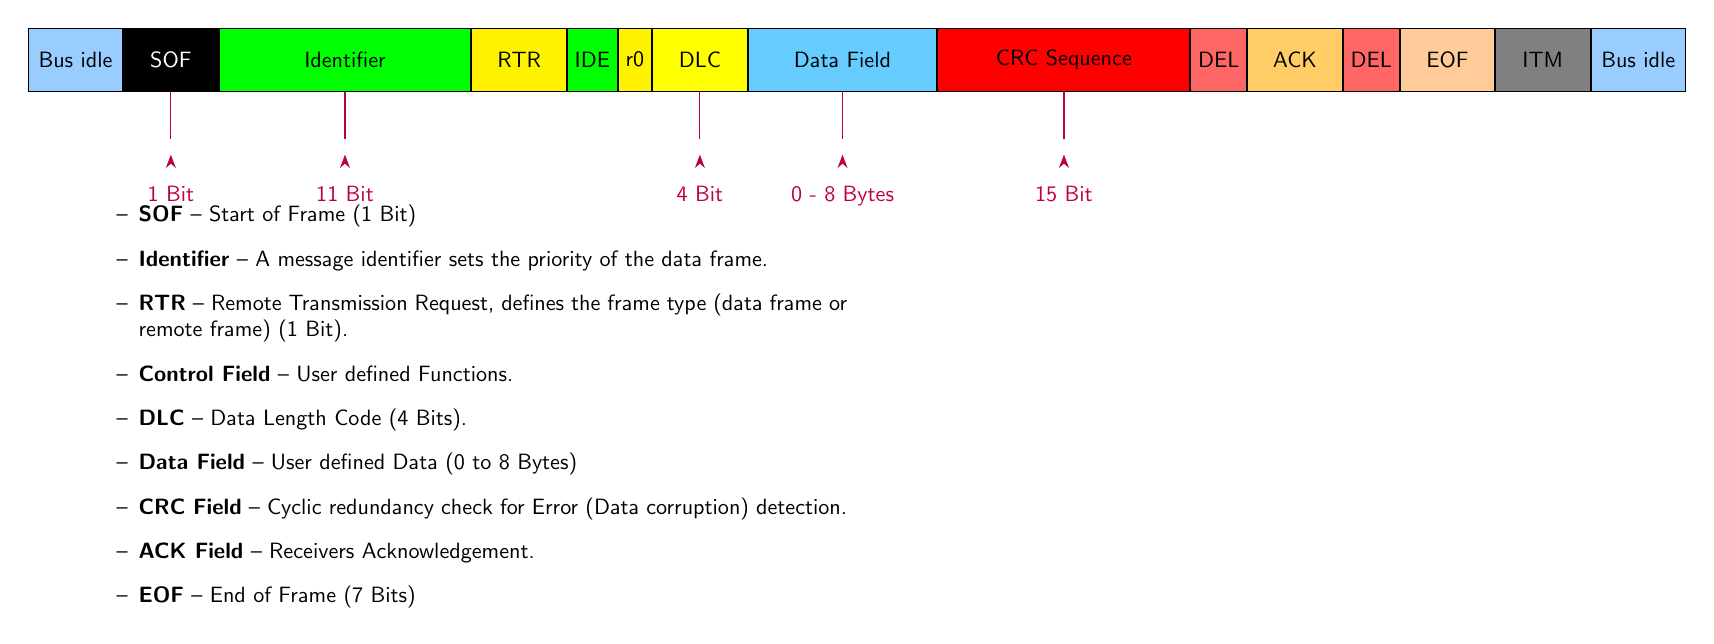
\begin{tikzpicture}[font=\sffamily, scale=0.8, transform shape, node distance=0cm and 0.5cm]

    % Define the colors
    \definecolor{busidlecolor}{RGB}{153,204,255}
    \definecolor{crcseqcolor}{RGB}{255,0,0}
    \definecolor{ackcolor}{RGB}{255,204,102}
    \definecolor{dlcolor}{RGB}{255,255,0}
    \definecolor{datacolor}{RGB}{102,204,255}
    \definecolor{delimitercolor}{RGB}{255,102,102}
    \definecolor{eofcolor}{RGB}{255,204,153}

    % Nodes
    \node[draw, fill=busidlecolor, minimum width=1.5cm, minimum height=1cm] (busidle1) {Bus idle};
    \node[draw, fill=black, text=white, minimum width=1.5cm, minimum height=1cm, right=0cm of busidle1] (sof) {SOF};
    \node[draw, fill=green, minimum width=4cm, minimum height=1cm, right=0cm of sof] (identifier) {Identifier};
    \node[draw, fill=yellow, minimum width=1.5cm, minimum height=1cm, right=0cm of identifier] (rtr) {RTR};
    \node[draw, fill=green, minimum width=0.5cm, minimum height=1cm, right=0cm of rtr] (ide) {IDE};
    \node[draw, fill=yellow, minimum width=0.5cm, minimum height=1cm, right=0cm of ide] (r0) {r0};
    \node[draw, fill=dlcolor, minimum width=1.5cm, minimum height=1cm, right=0cm of r0] (dlc) {DLC};
    \node[draw, fill=datacolor, minimum width=3cm, minimum height=1cm, right=0cm of dlc] (data) {Data Field};
    \node[draw, fill=crcseqcolor, minimum width=4cm, minimum height=1cm, right=0cm of data] (crc) {CRC Sequence};
    \node[draw, fill=delimitercolor, minimum width=0.5cm, minimum height=1cm, right=0cm of crc] (crcdel) {DEL};
    \node[draw, fill=ackcolor, minimum width=1.5cm, minimum height=1cm, right=0cm of crcdel] (ack) {ACK};
    \node[draw, fill=delimitercolor, minimum width=0.5cm, minimum height=1cm, right=0cm of ack] (ackdel) {DEL};
    \node[draw, fill=eofcolor, minimum width=1.5cm, minimum height=1cm, right=0cm of ackdel] (eof) {EOF};
    \node[draw, fill=gray, minimum width=1.5cm, minimum height=1cm, right=0cm of eof] (itm) {ITM};
    \node[draw, fill=busidlecolor, minimum width=1.5cm, minimum height=1cm, right=0cm of itm] (busidle2) {Bus idle};

    % Arrows for bits
    \draw[-{Stealth}, purple] (sof.south) -- ++ (0,-0.75) node[midway, below=1cm of sof] {1 Bit} ++(0,-0.25);
    \draw[-{Stealth}, purple] (identifier.south) -- ++(0,-0.75) node[midway, below=1cm of identifier] {11 Bit} ++(0,-0.25);
    \draw[-{Stealth}, purple] (dlc.south) -- ++(0,-0.75) node[midway, below=1cm of dlc] {4 Bit} ++(0,-0.25);
    \draw[-{Stealth}, purple] (data.south) -- ++(0,-0.75) node[midway, below=1cm of data] {0 - 8 Bytes} ++(0,-0.25);
    \draw[-{Stealth}, purple] (crc.south) -- ++(0,-0.75) node[midway, below=1cm of crc] {15 Bit} ++(0,-0.25);

    % Labels
    \node[below=5cm of busidle1, align=left, anchor=west] (labels) {
        \begin{minipage}{\textwidth}
            \begin{itemize}
                \item[--] \textbf{SOF} – Start of Frame (1 Bit)
                \item[--] \textbf{Identifier} – A message identifier sets the priority of the data frame.
                \item[--] \textbf{RTR} – Remote Transmission Request, defines the frame type (data frame or remote frame) (1 Bit).
                \item[--] \textbf{Control Field} – User defined Functions.
                \item[--] \textbf{DLC} – Data Length Code (4 Bits).
                \item[--] \textbf{Data Field} – User defined Data (0 to 8 Bytes)
                \item[--] \textbf{CRC Field} – Cyclic redundancy check for Error (Data corruption) detection.
                \item[--] \textbf{ACK Field} – Receivers Acknowledgement.
                \item[--] \textbf{EOF} – End of Frame (7 Bits)
            \end{itemize}
        \end{minipage}
    };

\end{tikzpicture}

\end{document}
